
\section{Higher-order methods for the advection equation}
\label{sec:ho-intro}

Chapter~\ref{ch:advection} introduced numerical methods for the linear
advection equation
\begin{equation}
\label{eq:ho-advect}
a_t + u a_x = 0
\end{equation}
that were first or second order in space. The advantages of using numerical
methods that are higher order can be large, especially when in regions where
the flow is smooth. However, these must be balanced against the additional
computational cost and complexity. In addition, many higher order methods do no
better than second order methods in cases with discontinuities.

\section{Finite difference methods}
\label{sec:ho-fd}

\subsection{The problem with higher-order finite volume methods}

The finite volume approach outlined in chapter~\ref{ch:fv}
%\todo{label missing in fv tex file?}
matches the physics of hyperbolic balance
laws perfectly, by maintaining the conservation of appropriate quantities using
the fluxes through the surfaces of each control volume or computational cell.
However, this leads to significant computational costs and complexities when
going beyond second order methods.

The inter-cell fluxes are computed by integrals over the face of the
computational cell. In one dimension the face is a single point and the
integral needs the flux evaluated at a single point, as in
equation~\ref{eq:consup}. In higher dimensions the face is one dimensional
(e.g., a line) or two dimensional (e.g., a square) and so the integral must be
approximated by evaluating the flux at \emph{multiple} points. If we use Gauss
quadrature, this means that a third order method would require at least two
flux evaluations per face in two dimensions, and typically four evaluations per
face in three dimensions.

As well as the additional computational cost, there is also typically an
additional restriction on the timestep. Intuitively this can be seen by
thinking about the flux evaluations again. We fix the values either side of the
cell boundary in order to compute the flux at one point.  The timestep
restriction is given by the time it take for information to propagate from a
different flux evaluation point, which would change the information available.
As we need to compute the flux at more points within the cell faces, the
distance between points where the flux is evaluated goes down, reducing the
time it takes for information to propagate from one point to another.

\subsection{Finite differences}

The conservative finite difference method starts from the endpoint for finite
volume methods, by considering the update formula~\eqref{eq:consup}
%\todo{is this the right equation to ref? Don't think it's labelled?}
\begin{equation}
\tag{\ref{eq:consup}}
\frac{\partial \langle \Uc\rangle_{i}}{\partial t} =
  - \frac{1}{\Delta x} \left \{ \Fb_{i+\myhalf} -
                                \Fb_{i-\myhalf} \right \}.
\end{equation}
In the finite difference method a interpretation used is different. We are now
thinking of
\begin{equation}
  \label{eq:fd-deriv}
  \frac{1}{\Delta x} \left \{ \Fb_{i+\myhalf} -
                                \Fb_{i-\myhalf} \right \}
\end{equation}
as representing a direct approximation to the derivative of the flux at $x_i$.
In particular, we are \emph{not} thinking of $\Fb_{i+\myhalf}$ as being
directly linked to the flux. Crucially the update still ensures global
conservation, as the ``flux'' term is re-used for neighbouring points in the
same way as in the finite volume case.

When we combine this viewpoint with the Method of Lines approach in
section~\ref{adv:sec:mol_2d}, the implementation of a high-order finite boils
down to
\begin{itemize}
  \item using a high-order time integration scheme (such as a high order
  Runge-Kutta method);
  \item finding a way that the finite difference in equation~\eqref{eq:fd-deriv}
  approximates the derivative of the flux both stably, and to a sufficiently
  high order.
\end{itemize}

\section{WENO reconstruction}
\label{sec:WENO}

\begin{figure}
  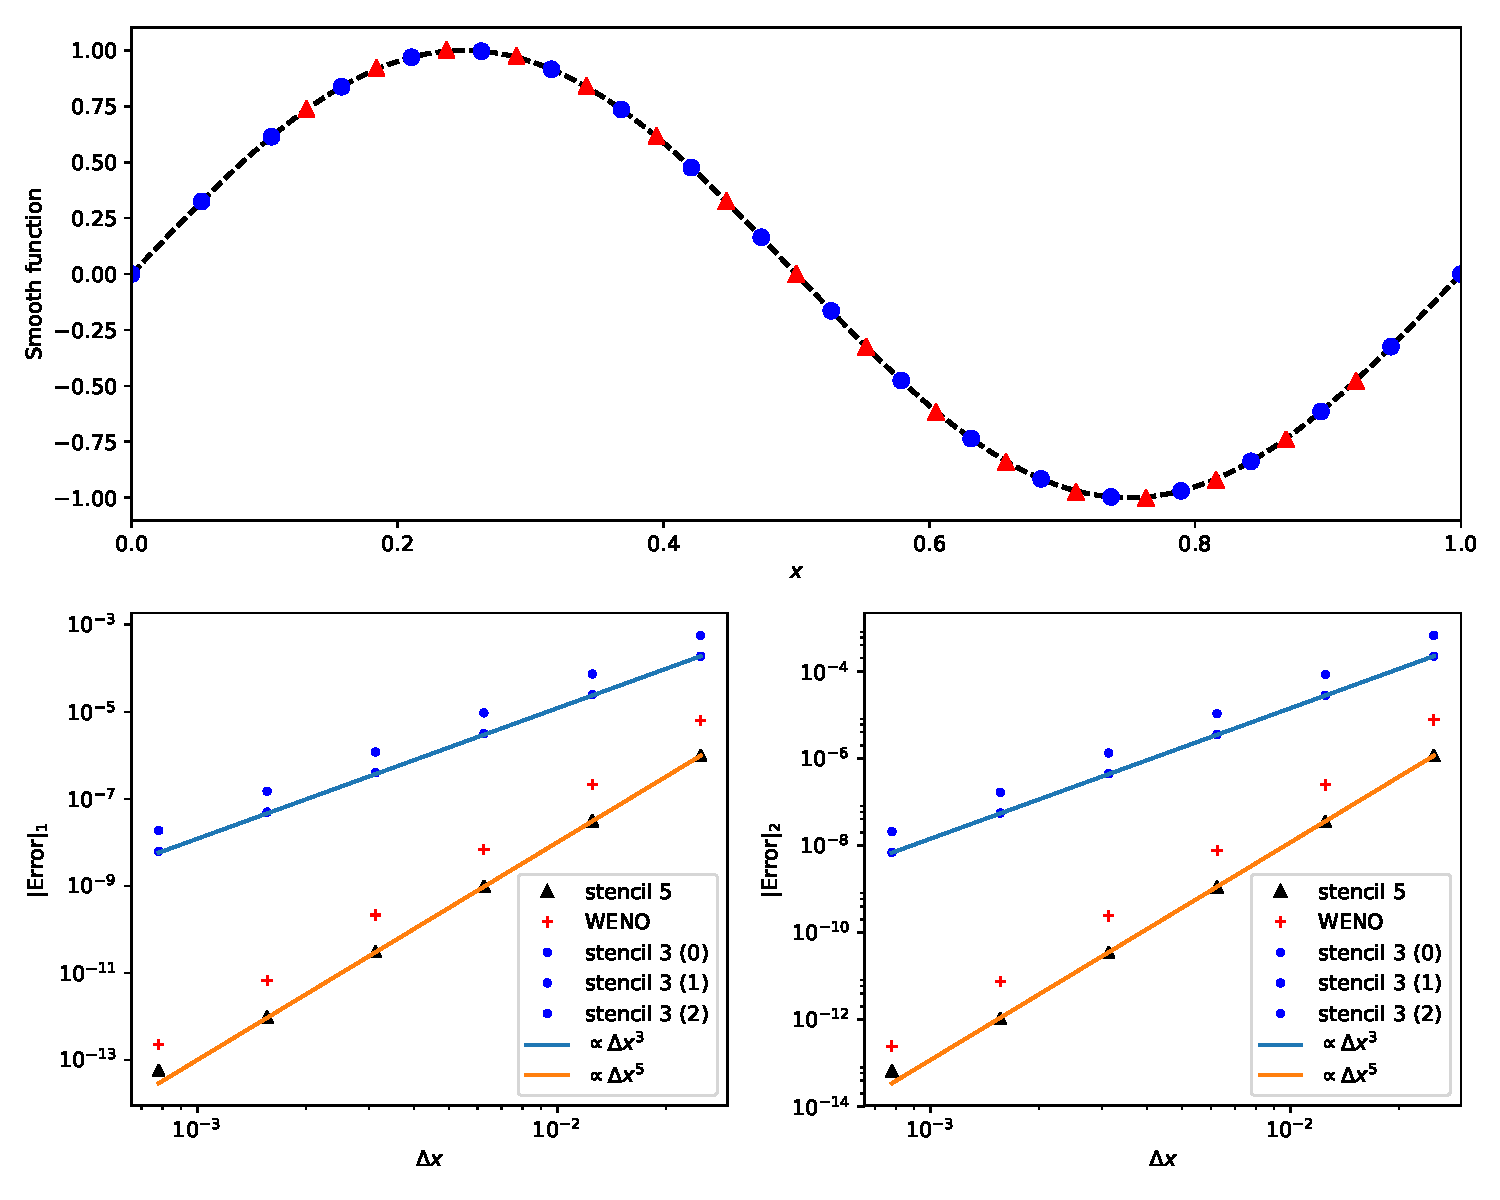
\includegraphics[width=0.96\linewidth]{weno-convergence}
  \caption[Convergence rate of high-order reconstructions]{A smooth sine function is reconstructed on the unit interval from the (integral-average) data, at the blue circles in the top plot, to the right, at the red triangles in the top plot. The convergence rate with grid resolution for the 5 point stencil of equation~\eqref{eq:weno-advection-5pt} and the 3 point stencils of equation~\eqref{eq:weno-advection-3pt} are shown to match expectations in the bottom plots. The error from the WENO reconstruction described in section~\ref{sec:WENO-algorithm} is, on this smooth function, converging with the expected order but larger in magnitude.}
  \label{fig:weno-convergence}
\end{figure}

For the advection equation with constant advection speed $u$, our higher-order
method requires us to find a high-order approximation to $a_{i+\myhalf}$. If we
considered the five points $a_{j}, j \in [i-2, \dots, i+2]$ then we could use
the information from all five of these points to approximate $a_{i+\myhalf}$ as
\begin{equation}
  \label{eq:weno-advection-5pt}
  a^{(\text{Fifth})}_{i+\myhalf} = \tfrac{1}{60} \left( 2 \langle q \rangle_{i-2} - 13 \langle q \rangle_{i-1} + 47 \langle q \rangle_{i} + 27 \langle q \rangle_{i+1} - 3 \langle q \rangle_{i+2} \right) + {\cal O}(\Delta x^5).
\end{equation}
Alternatively we could use only three of the points, in three different ways:
\begin{subequations}
  \label{eq:weno-advection-3pt}
  \begin{align}
    a^{(\text{Third}, 2)}_{i+\myhalf} &= \tfrac{1}{6} \left( 2 \langle q \rangle_{i-2} - 7 \langle q \rangle_{i-1} + 11 \langle q \rangle_{i} \right) + {\cal O}(\Delta x^3), \\
    a^{(\text{Third}, 1)}_{i+\myhalf} &= \tfrac{1}{6} \left( - \langle q \rangle_{i-1} + 5 \langle q \rangle_{i} + 2 \langle q \rangle_{i+1} \right) + {\cal O}(\Delta x^3), \\
    a^{(\text{Third}, 0)}_{i+\myhalf} &= \tfrac{1}{6} \left( 2 \langle q \rangle_{i} + 5 \langle q \rangle_{i+1} - \langle q \rangle_{i+2} \right) + {\cal O}(\Delta x^3).
  \end{align}
\end{subequations}

Which is better? The five point stencil gives higher order accuracy, but
includes information from both sides of the point. This ignores information from
the characteristics and, near discontinuities, will lead to Gibbs oscillations.
The three point stencils give lower accuracy. However, they give us the
flexibility to choose a stencil to avoid discontinuities, possibly using the
characteristic information. The advantages of the higher-order methods are illustrated by reconstructing a smooth function in figure~\ref{fig:weno-convergence}. The disadvantages of using a fixed stencil are illustrated by reconstructing a non-smooth function in figure~\ref{fig:weno-weights}.


\begin{exercise}[ENO stencils]
{Check that equations~\eqref{eq:weno-advection-5pt} and
\eqref{eq:weno-advection-3pt} give the claimed order of accuracy results.}
\end{exercise}

The method of choosing the ``best'' stencil (to avoid discontinuities as far as
possible) is called \emph{Essentially Non-Oscillatory} (ENO) reconstruction. It
is not as accurate as it could be given the size of the stencil it uses, and
the logical branches required to find the ``best'' stencil can reduce
computational performance.

An alternative that avoids the problems of ENO schemes are the \emph{Weighted}
ENO, or WENO, schemes. These use a combination of the possible ENO stencils to
reconstruct $a_{i+\myhalf}$. This relies on the observation that there are
constants $C_k$ such that, for example,
\begin{equation}
  \label{eq:WENO-C-weights}
  a^{(\text{Fifth})}_{i+\myhalf} = \sum_{k=0}^{2} C_k a^{(\text{Third}, r)}_{i+\myhalf}.
\end{equation}

\begin{exercise}[WENO weights]
{Check that the constants $C_0 = \tfrac{3}{10}, C_1 = \tfrac{3}{5}, C_2 =
\tfrac{1}{10}$ make equation~\eqref{eq:WENO-C-weights} consistent with
equations~\eqref{eq:weno-advection-5pt} and \eqref{eq:weno-advection-3pt}.}
\end{exercise}

The WENO methods work by retaining the sum over all stencils as in
equation~\eqref{eq:WENO-C-weights}, but adjusting the weights to avoid
oscillations. Ideally, in regions where the $a^{(0,1)}$ stencils include a
shock but the $a^{(2)}$ stencil does not the weights should be $\tilde{C}_0 = 0
= \tilde{C}_1$ and $\tilde{C}_2 = 1$. In order for this sum to make sense we
will need the weights to add to $1$.

\subsection{WENO algorithm}
\label{sec:WENO-algorithm}

\begin{figure}
  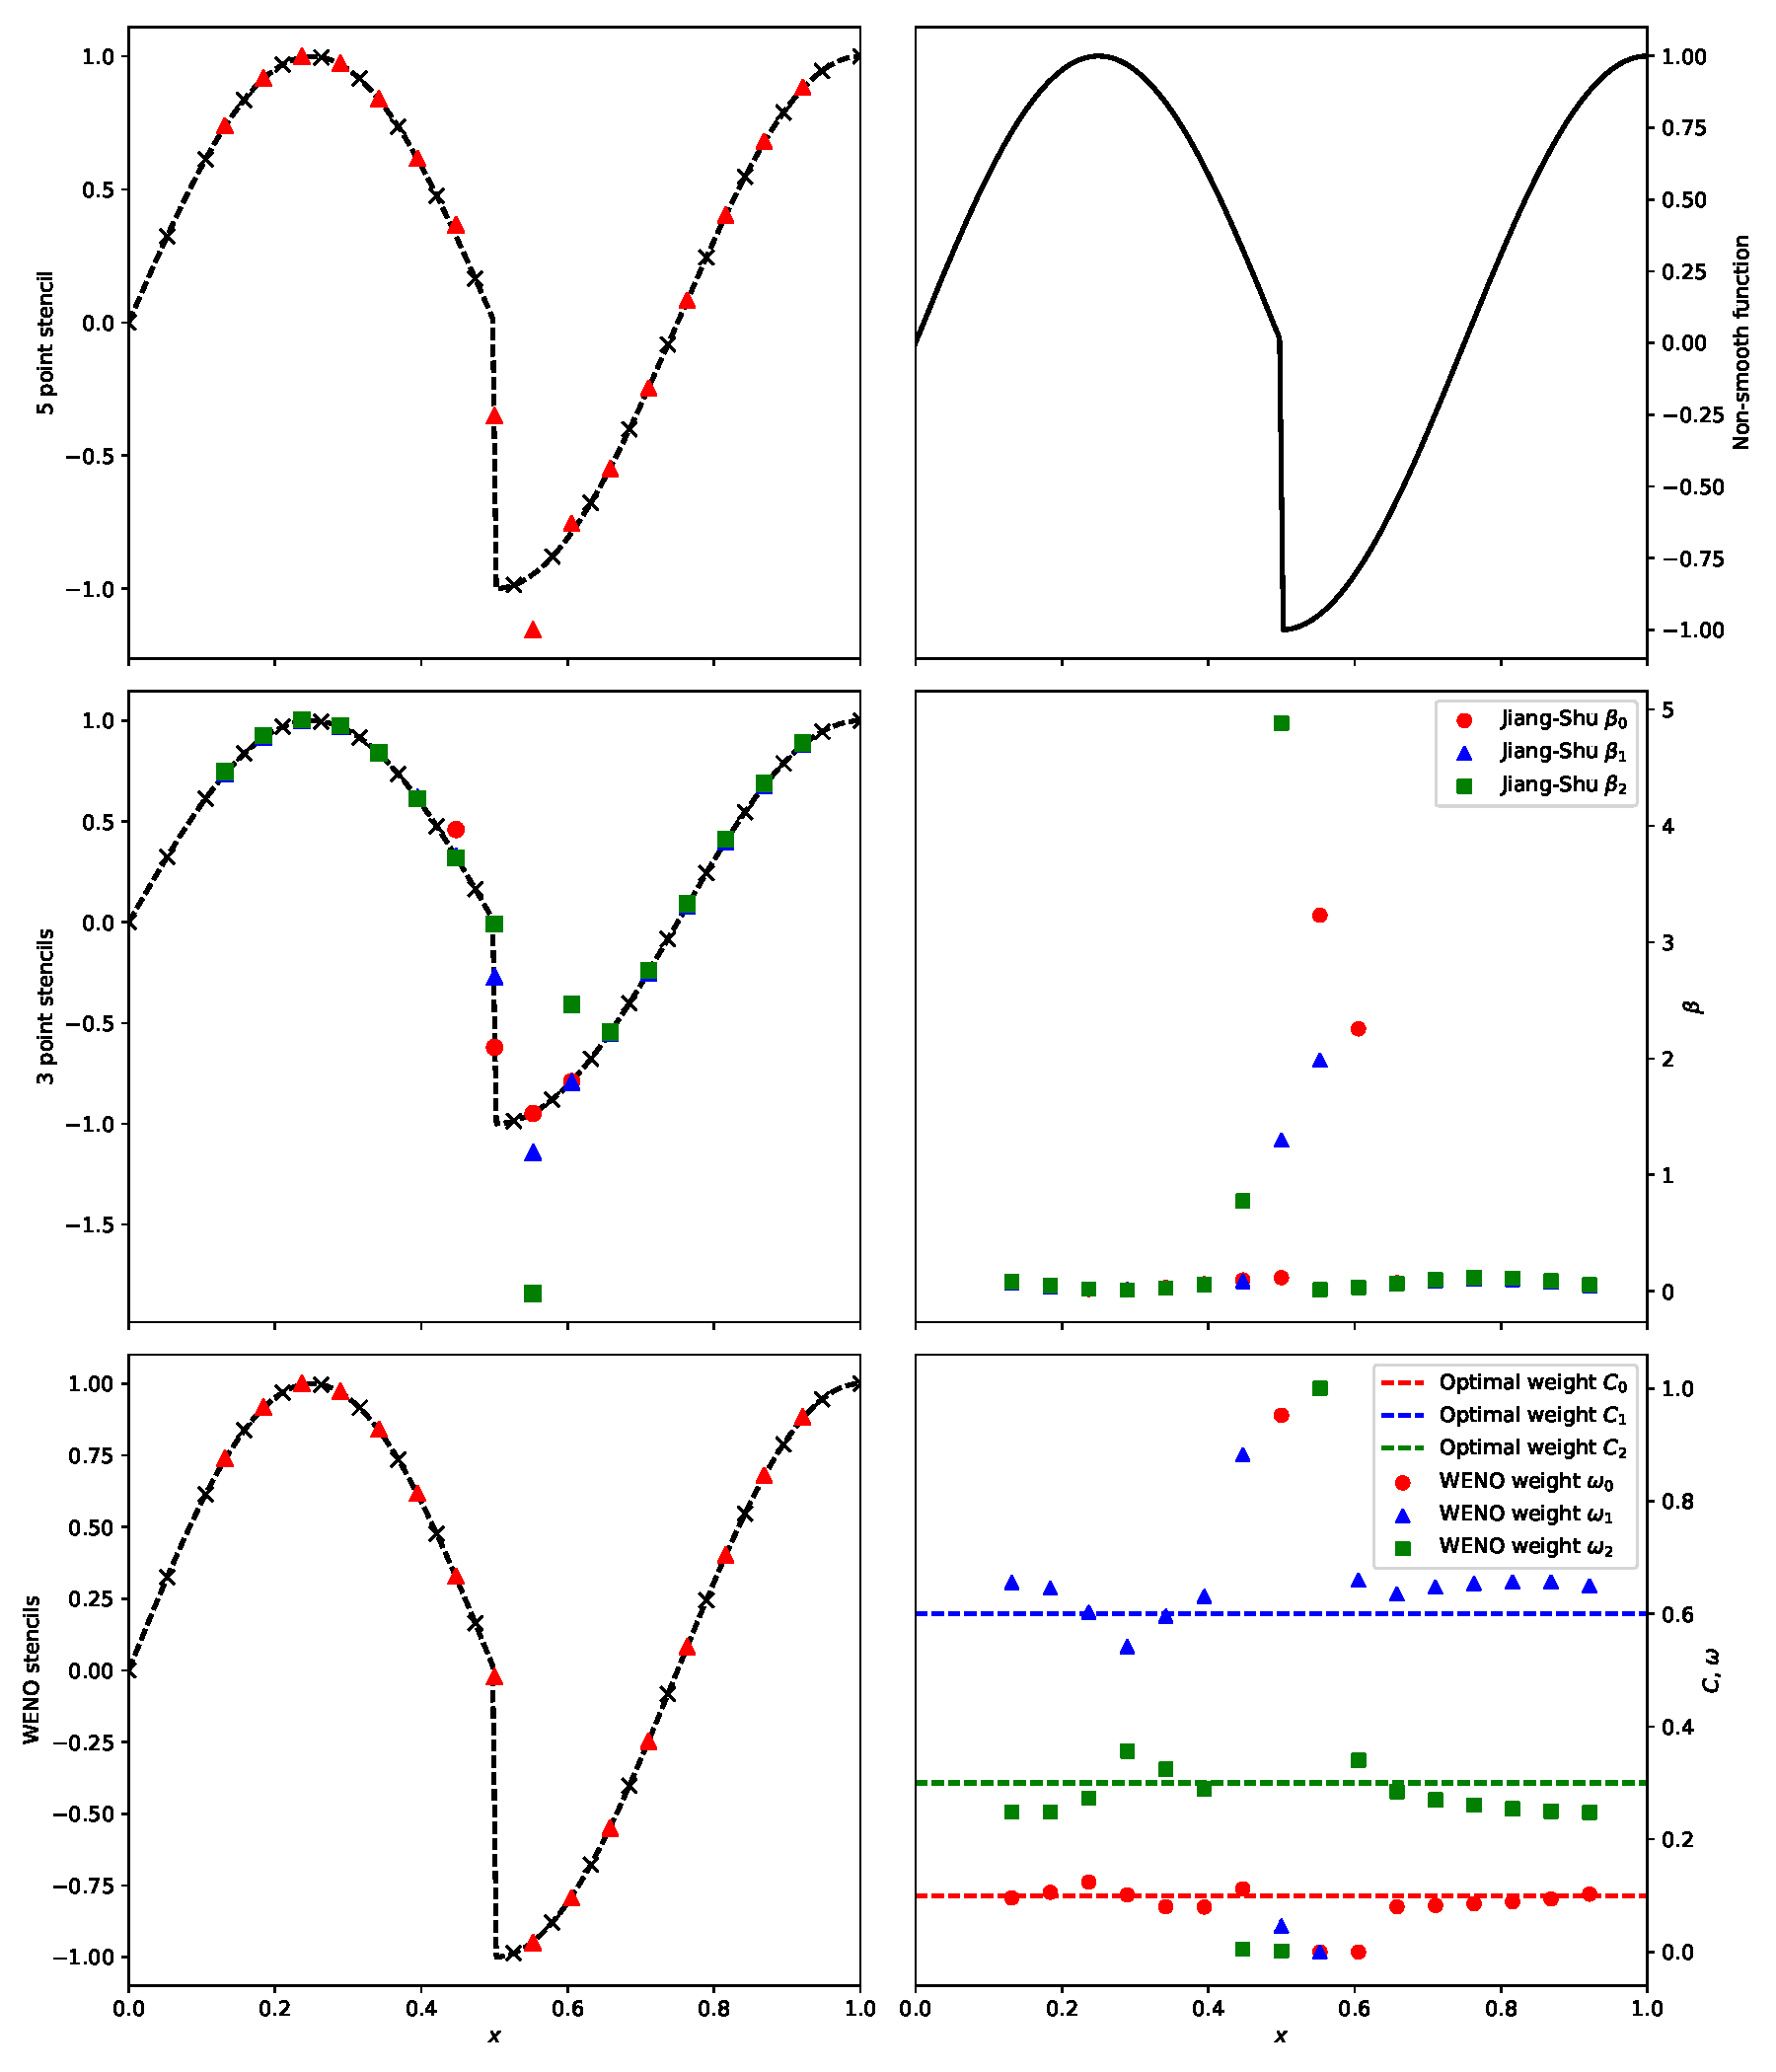
\includegraphics[width=0.96\linewidth]{weno-weights}
  \caption[WENO reconstruction and weights]{A non-smooth function is reconstructed on the unit interval. The 5 point stencil of equation~\eqref{eq:weno-advection-5pt} and the 3 point stencils of equation~\eqref{eq:weno-advection-3pt} both show oscillations near the discontinuity, whilst the WENO reconstruction does not. The WENO algorithm depends on measuring the smoothness of the function. The Jiang-Shu smoothness indicators $\beta$ are mostly zero, but spike near the discontinuity. This feeds into the weight $\omega$ that the WENO algorithm gives to each 3 point stencil it uses. Away from the discontinuity the weights revert to the optimal $C$ weights, but near the discontinuity a single $\omega$ weight dominates meaning only a single 3 point stencil is used.}
  \label{fig:weno-weights}
\end{figure}

We can now write out the full WENO algorithm of order $(2 r - 1)$. The constant
$r$ sets the size of the individual stencils as well as the (optimal) order of
the scheme. This section uses the notation of Gerolymos et al., and we will drop the integral average notation (so $\langle q \rangle_i$ will be denoted $a_i$).

First compute the individual stencils
\begin{equation}
  \label{eq:weno-stencils}
  a_{r, k, i+\myhalf} = \sum_{\ell=0}^{r-1} A_{r, k, \ell} A_{i+k-\ell}, \quad k = 0, \dots, r-1.
\end{equation}
Here the $A_{r, k, \ell}$ terms are constants which, for given scheme accuracy
$r$ are needed to compute the $k^{\text{th}}$ stencil.

We then want to combine these individual stencils to compute the WENO result.
For this we write
\begin{equation}
  \label{eq:weno-reconstruction}
  a_{r, WENO, i+\myhalf} = \sum_{k=0}^{r-1} \omega_{r, k, i+\myhalf} a_{r, k, i+\myhalf}.
\end{equation}
Here the $\omega_{r, k, i+\myhalf}$ terms are the weights that vary from point
to point. They must sum to one, so that we have a convex combination of the
stencils:
\begin{equation}
  \label{eq:weno-convex}
  \sum_{k=1}^{r-1} \omega_{r, k, i+\myhalf} = 1.
\end{equation}
We also want the weights to match the \emph{optimal} weights $C_{r, k}$ in
smooth regions. The optimal weights are defined such that
\begin{equation}
  \label{eq:weno-optimal}
  a_{r, WENO, i+\myhalf} = \sum_{k=0}^{r-1} C_{r, k} a_{r, k, i+\myhalf}
\end{equation}
is accurate to order ${\cal O}(\Delta x^{(2 r - 1)})$ when $q$ is smooth.

The \emph{choice} of how to get from the optimal weights $C_{r, k}$ to the
nonlinear weights $\omega_{r, k, i+\myhalf}$ defines the WENO scheme. The
standard choice of Jiang and Shu is to introduce a measure of the smoothness of
the $k^{\text{th}}$ stencil by computing the sum of the integral averages of
its derivatives from order $1$ up to order $2 r - 1$. For practical
implementation purposes this means computing the \emph{smoothness indicators}
$\beta_{r, k, i+\myhalf}$ as
\begin{equation}
  \label{eq:weno-smoothness}
  \beta_{r, k, i+\myhalf} = \sigma_{r, k, \ell, m} a_{i+k-\ell} a_{i+k-m}.
\end{equation}
The terms $\sigma_{r, k, \ell, m}$ are pre-computed constants which give the
coefficients in the quadratic form for the $k^{\text{th}}$ stencil of width $r$
in the reconstruction. These smoothness indicators are non-negative, and will
be large when the derivatives are large in magnitude. The Jiang and Shu weights
are then set by
\begin{subequations}
  \label{eq:weno-nonlinear-weights}
  \begin{align}
    \label{eq:weno-nonlinear-weights-omega}
    \omega_{r, k, i+\myhalf} &= \frac{\alpha_{r, k, i+\myhalf}}{\sum_{k=0}^{r-1} \alpha_{r, k, i+\myhalf}}, \\
      \label{eq:weno-nonlinear-weights-alpha}
    \alpha_{r, k, i+\myhalf} &= \frac{C_{r, k}}{\epsilon + \beta_{r, k, i+\myhalf}^2}.
  \end{align}
\end{subequations}
Here $\epsilon$ is a small number introduced to avoid division-by-zero problems.
The form of $\omega_{r, k, i+\myhalf}$ in
equation~\eqref{eq:weno-nonlinear-weights-omega} guarantees that the convex sum
condition in equation~\eqref{eq:weno-convex} holds. The form of $\alpha_{r, k,
i+\myhalf}$ ensures that when all the smoothness indicators $\beta_{r, k,
i+\myhalf}$ are the same magnitude the weights $\omega_{r, k, i+\myhalf}$ will
match the optimal weights $C_{r, k}$, but when a smoothness indicator is large
(i.e., when the associated stencil has large derivatives, typically associated
with discontinuities), the contribution of its associated stencil will be small.
An example of this is shown in figure~\ref{fig:weno-weights}.

Finally, we note that this method has reconstructed $a_{i+\myhalf}$ from the
left. For the advection equation case where the advection speed $u$ is positive
this is all we need: the characteristic information tells us that we should use
this reconstruction. In the case where the advection speed is negative we
should reconstruct from the right. In the implementation it is easiest to
implement only one reconstruction direction and pass the data in in reverse
order.


\begin{exercise}[WENO reconstruction]
{Taking the values for the $C$, $A$ and $\sigma$ constants from Gerolymos et
al.\ or Shu's review, construct a WENO reconstruction method for $r=2$. Check
your results on smooth and non-smooth functions.}
\end{exercise}

\section{Nonlinear equations and flux-splitting}

%\todo{This shouldn't go here - probably belongs after the Euler section - but for now this keeps all the WENO stuff together}
%\todo{Also note that I haven't followed the notation of the rest of the notes as I was too lazy to work out what it was.}

For a nonlinear scalar conservation law
\begin{equation}
  \label{eq:scalar_conslaw}
  u_t + f(u)_x = 0
\end{equation}
the WENO method above does not work, as we have assumed the characteristic
information travels in one direction only. We have also reconstructed the
variable $q$ and from that constructed the ``flux'' which we feed into the
differencing formula of equation~\eqref{sec:ho-fd} to update the solution: this
will not work either.

In the nonlinear case, we instead reconstruct the \emph{flux} directly. That
is, given the state $u_i$ at location $x_i$, we compute the flux $f_i = f(u_i)$
and reconstruct the flux $f_{i+\myhalf}$ using the WENO reconstruction above.

This has the significant problem that we have no characteristic information for
the flux: does it propagate to the left or to the right? To get around this we
introduce \emph{flux splitting}. We write
\begin{equation}
  \label{eq:flux-splitting}
  f(u) = f^{(+)}(u) + f^{(-)}(u)
\end{equation}
where we choose the functions such that the information contained in $f^{(+)}$
propagates to the right and that in $f^{(-)}$ propagates to the left. There are
many ways of doing this, but the simplest is the \emph{Lax-Friedrichs} flux
splitting
\begin{equation}
  \label{eq:lf-flux-split}
  f^{(\pm)}(u) = \tfrac{1}{2} \left( f(u) \pm \alpha u \right)
\end{equation}
where $\alpha \ge \max | \partial_u f |$. With $\alpha$ being larger than the maximum propagation speed, this means that
\begin{equation}
  \label{eq:lf-flux-split-speeds}
  \partial_u f^{(+)} \ge 0, \quad \partial_u f^{(-)} \le 0,
\end{equation}
and the characteristic information contained in $f^{(\pm)}$ will propagate as required.

The simplest flux-split algorithm is then
\begin{enumerate}
  \item Compute the maximum characteristic speed $\alpha$ over the entire computational grid;
  \item Compute the split fluxes $f^{(\pm)}$ from equation~\eqref{eq:lf-flux-split};
  \item Reconstruct $f^{(+)}$ to the right using, e.g., the WENO algorithm of section~\ref{sec:WENO};
  \item Reconstruct $f^{(-)}$ to the left using the same method;
  \item Compute $f_{i+\myhalf} = f^{(+)}_{i+\myhalf} + f^{(-)}_{i+\myhalf}$;
  \item Update the state using equation~\eqref{eq:consup}.
\end{enumerate}

\subsection{Extensions}

Extending to multiple dimensions using dimensional splitting. From the
finite-difference form there are no transverse Riemann problems to solve. From
using the Method of Lines there is no issue about ordering the dimensional
sweeps: the updates in each direction are computed separately but applied
together in the time integrator. This formally retains the high-order accuracy
but can lose significant absolute accuracy -- compare the advection of a
top-hat function with lower order methods using transverse Riemann problem
solutions.

The global Lax-Friedrichs flux splitting above can be excessively diffusive. A
local Lax-Friedrichs flux splitting, where $\alpha$ is computed at each point
by maximising over the characteristic speed within the stencil at that point, is
less diffusive but slightly more expensive. Roe-style flux splittings are
possible but not always stable.

When dealing with nonlinear systems the flux split method generalizes directly.
The simplest method is to compute $\alpha$ by maximizing over all
characteristics. It is possible to significantly reduce the diffusive nature of
the flux splitting by reconstructing the \emph{characteristic} fluxes and using
a local computational of the specific characteristic speed. This requires both
significant additional computational expense and the knowledge of the spectral
information (left and right eigenvectors of the Jacobian matrix).
